\documentclass{beamer}

\usepackage{pri}
%\usepackage{comment}

\graphicspath{{./}{figures/}{figures/14-web-crawling-figs/}} 

%
% slides baseados nos de 
% By Filippo Menczer
% Indiana University School of Informatics
% in Web Data Mining by Bing Liu 
% Springer, 2007 



\subtitle{Web Crawling}


\begin{document}

\maketitle


% ------------------------------------------------------------

\begin{frame} \frametitle{Bibliography}

    \begin{block}{}
        \begin{itemize}

       \item \href{http://www.cs.uic.edu/~liub/WebMiningBook.html}{Bing Liu, Web Data Mining: Exploring Hyperlinks, Contents, and
         Usage Data, 2nd edition}.  Chapter 8

       \item most slides based on presentation by Filippo Menczer, Indiana University School of Informatics
    
\end{itemize}
    \end{block}

\end{frame}


\begin{frame} \frametitle{Outline}

    \begin{itemize}

       \item  Motivation and taxonomy of crawlers
       \item  Basic crawlers and implementation issues
       \item  Universal crawlers
       \item  Preferential (focused and topical) crawlers
       %\item  Evaluation of preferential crawlers
       \item  Crawler ethics and conflicts
       %\item  New developments: social, collaborative, federated crawlers

\end{itemize}

\end{frame}


\section{Crawling}

\begin{frame} \frametitle{Names}

 \begin{columns}[T]
    \begin{column}{0.5\textwidth}

    \begin{itemize}
    \item Crawler
    \item Spider
    \item Robot (or bot)
    \item Web agent
    \item Wanderer, worm, ...
    \end{itemize}
\end{column}

\begin{column}{.5\textwidth}
 
\includegraphics [width=.9\textwidth]{google-bot-logo-with-bot} 
\end{column}
\end{columns}

\begin{block}{instances:}
googlebot, scooter (altavista), slurp (yahoo), msnbot, ...
\end{block}

\end{frame}

\begin{frame} \frametitle{Why Develop a Crawler?}

    \begin{itemize}

\item Support universal search engines (Google, Yahoo, Bing, Ask, etc.)
\item Vertical (specialized) search engines, e.g. news, shopping, papers, recipes, reviews, etc.
\item Business intelligence: keep track of potential competitors, partners
\item Monitor Web sites of interest
\item Evil: harvest emails for spamming, phishing ...

%\item ...Can you think of some others? ...

\end{itemize}

\end{frame}

\begin{frame} \frametitle{The Crawler and the Search Engine}

 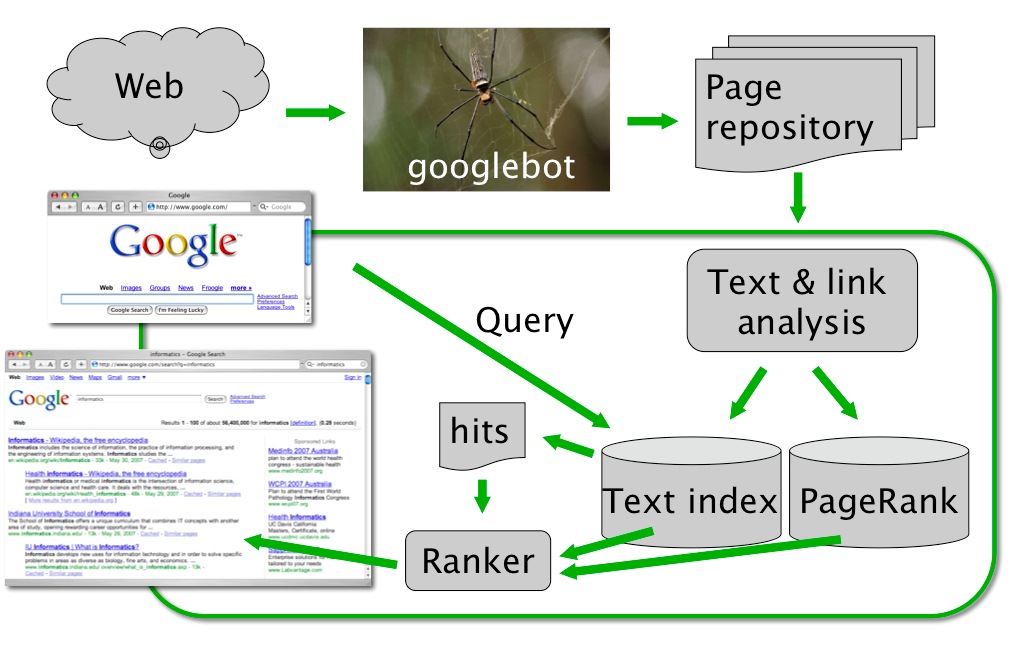
\includegraphics [width=10cm]{crawler-search-engine} 

\end{frame}


\section{Basic Crawlers}


\begin{frame} \frametitle{Basic Crawler}

  \begin{columns}[T]
    \begin{column}{0.5\textwidth}

    \begin{itemize} 
    \item  This is a \textbf{sequential crawler}
    \item  Seeds can be any list of starting URLs
    \item  Order of page visits is determined by \textbf{frontier} data structure
    \item  Stop criterion can be anything

    \end{itemize}

    \end{column}
    \begin{column}{0.5\textwidth}
      \hfill 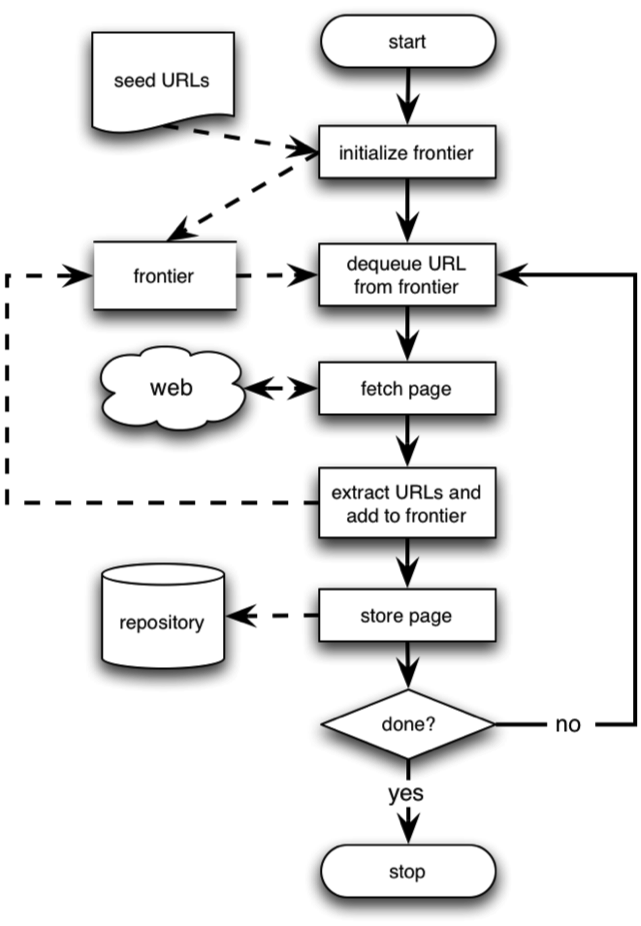
\includegraphics[width=5cm]{crawler-flow-chart}
    \end{column}


\end{columns}

\end{frame}

\begin{frame} \frametitle{BFS vs DFS Graph Traversal}
 
\begin{columns}[T]
    \begin{column}{0.5\textwidth}

Breadth First Search

    \begin{itemize} 
    \item Implemented with QUEUE (FIFO) 
    \item Finds pages along shortest paths
    \item If we start with ``good'' pages, this keeps us close; maybe
      other good stuf...
    % \item order tends to correlate with \textbf{PageRank}
     \end{itemize}

 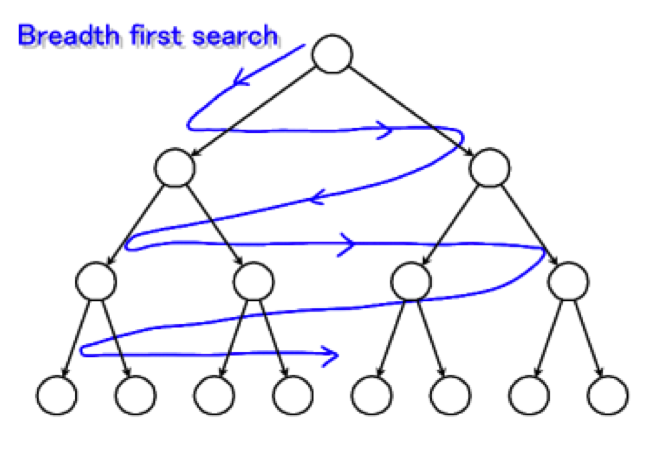
\includegraphics[width=5cm]{BFS}

    \end{column}
    \begin{column}{0.5\textwidth}


Depth First Search

    \begin{itemize} 
    \item Implemented with STACK (LIFO)
    \item Wander away (``lost in cyberspace'')
      \end{itemize}

 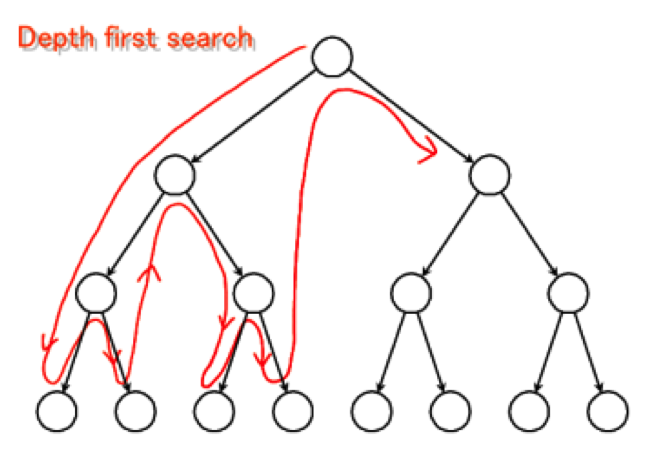
\includegraphics[width=5cm]{DFS}


   \end{column}
   
\end{columns}


\end{frame}

\begin{frame}[fragile] \frametitle{Main Loop of a Basic Crawler }
 
\begin{verbatim}
frontier is a queue
frontier = read_seeds(file)

while length(frontier) > 0 & total_collected < max

    next_link = shift frontier

    page = fetch(next_link)

    add_to_index(page)

    links = extract_links(page, next_link)

    push frontier, process(links)

\end{verbatim}

\end{frame}

\subsection{Implementation Issues}

\begin{frame} \frametitle{Implementation Issues}

\begin{itemize}

\item Don't want to fetch same page twice!
\begin{itemize}
\item Keep lookup table (hash or Bloomfilter) of visited pages
\item What if not visited but in frontier already?
\end{itemize}

\item The frontier grows very fast!
\begin{itemize}
\item May need to prioritize for large crawls
\end{itemize}

\item Fetcher must be robust! 
\begin{itemize}
\item Don't crash if download fails
\item Have a timeout mechanism
\item Don't overload servers
\end{itemize}

\item Determine file type to skip unwanted files
\begin{itemize}
\item Can try using extensions, but not reliable
\item Can issue HEAD HTTP commands to get \\ Content-Type (MIME)
  headers, but there is overhead of extra Internet requests
\end{itemize}

\end{itemize}

\end{frame}

\begin{frame} \frametitle{Implementation Issues: Fetching}
\begin{itemize}
\item  Get only the first 10-100 KB per page

\item Take care to detect and break {\bf redirection loops}

\item Soft fail for 
\begin{itemize}
\item timeout, 
\item server not responding,
\item file not found
\item ...other errors
\end{itemize}

\end{itemize}

\end{frame}


\begin{frame} \frametitle{Implementation Issues: Parsing HTML}

\begin{columns}[T]
\begin{column}{0.5\textwidth}
\begin{itemize}

\item HTML has the structure of a DOM (Document Object Model) tree

\item Unfortunately actual HTML is often incorrect in a strict syntactic sense
\begin{itemize}
\item Crawlers, like browsers, must be robust/forgiving
\item Fortunately there are tools that can help (e.g., HTML Tidy)
\end{itemize}
\item Must pay attention to HTML entities and unicode in text

\end{itemize}
\end{column}

\begin{column}{.5\textwidth}
      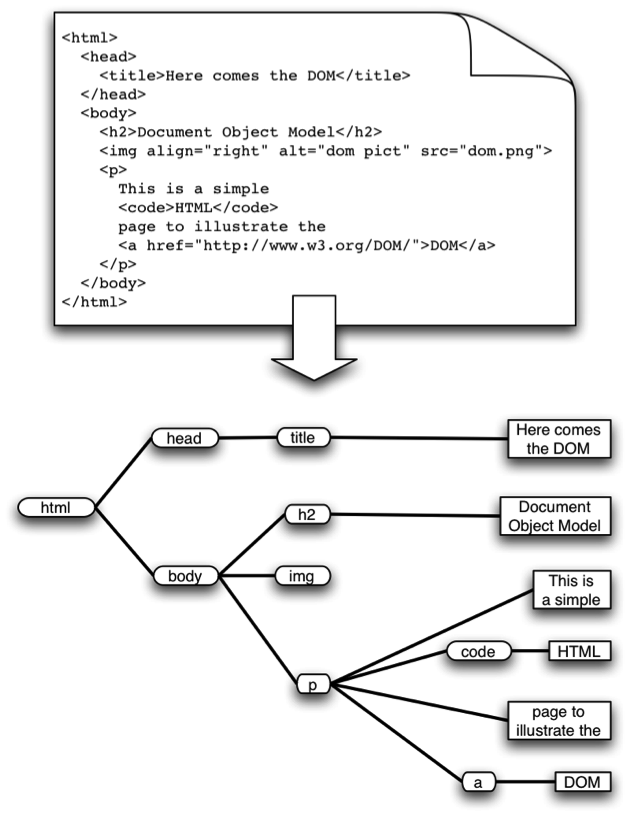
\includegraphics[width=4cm]{crawler-parsing}
\end{column}

\end{columns}

\end{frame}

\begin{frame} \frametitle{Implementation issues: Parsing Other Formats}


\begin{block}{What to do with other formats?}

\begin{itemize}
\item JavaScript, 
\item SVG, 
\item RSS, 
\item Flash,
\item ...

\end{itemize}

\end{block}

\end{frame}

\begin{frame} \frametitle{Implementation issues: Relative vs. Absolute URLs}


Crawler must translate relative URLs into absolute URLs

Need to obtain Base URL from HTTP header, or HTML Meta tag, or else current page path by default

\begin{block}{Examples:}
\begin{description}
\item[Base:] \url{http://www.cnn.com/linkto/}
\item [Relative URL:] \url{intl.html}
\item [Absolute URL:] \url{http://www.cnn.com/linkto/intl.html}
\item [Relative URL:] \url{/US/}
\item [Absolute URL:] \url{http://www.cnn.com/US/}
\end{description}
\end{block}

\end{frame}


\begin{frame} \frametitle{Implementation issues: URL canonicalization}

\begin{block}{ All of these:}

\url{http://www.cnn.com/TECH}

\url{http://WWW.CNN.COM/TECH/}

\url{http://www.cnn.com:80/TECH/}

\url{http://www.cnn.com/bogus/../TECH/}



\end{block}

\begin{block}{Are really equivalent to this canonical form:}
http://www.cnn.com/TECH/
\end{block}

In order to avoid duplication, the crawler must transform all URLs into canonical form

Definition of ``canonical'' is arbitrary, e.g.:
Could always include port, or only include port when not default

\end{frame}

\begin{frame} \frametitle{More on Canonical URLs}

Some transformations are trivial, for example:

\url{http://tecnico.ulisboa.pt/} 

\url{http://tecnico.ulisboa.pt}

\vspace{\baselineskip}

\url{http://tecnico.ulisboa.pt/index.html\#fragment}

\url{http://tecnico.ulisboa.pt/index.html}
\vspace{\baselineskip}

\url{http://tecnico.ulisboa.pt/dir1/./../dir2/}

\url{http://tecnico.ulisboa.pt/dir2/}
\vspace{\baselineskip}

\url{http://tecnico.ulisboa.pt/\%7Efil/}

\url{http://tecnico.ulisboa.pt/~fil/}
\vspace{\baselineskip}

\url{http://TECNICO.ULISBOA.PT/fil/}

\url{http://tecnico.ulisboa.pt/fil/}

\end{frame}


\begin{frame} \frametitle{More on Canonical URLs}

Other transformations require heuristic assumption about the intentions of the author or configuration of the Web server:

\begin{block}{Removing default file name}

\url{http://tecnico.ulisboa.pt/fil/index.html}

\url{http://tecnico.ulisboa.pt/fil/}

This is reasonable in general but would be wrong in this case because the default happens to be \url{default.asp} instead of \url{index.html}
\end{block}

\begin{block}{Trailing directory}

\url{http://tecnico.ulisboa.pt/fil}

\url{http://tecnico.ulisboa.pt/fil/}

This is correct in this case but how can we be sure in general that there isn't a file named ``fil'' in the root dir?
\end{block}

\end{frame}



\begin{frame} \frametitle{Implementation issues: Spider Traps}

Misleading sites: indefinite number of pages dynamically generated by CGI scripts 

Paths of arbitrary depth created using soft directory links and path rewriting features in HTTP server

\begin{block}{Heuristic defensive measures (the single option):}

\begin{itemize}
\item Check URL length; assume spider trap above some threshold, for example 128 characters
\item Watch for sites with very large number of URLs
\item Eliminate URLs with non-textual data types
\item May disable crawling of dynamic pages, if detected
\end{itemize}
\end{block}

\end{frame}

\begin{frame} \frametitle{Implementation issues: Page Repository}

\begin{description}
\item [Naive:] store each page as a separate file.
Can map URL to unique filename using a hashing function, e.g. MD5
This generates a huge number of files, which is inefficient from the storage perspective

\item [Better:] combine many pages into a single large file, using some XML markup to separate and identify them.
Must map URL to ${filename, page\_id}$
\end{description}

\begin{block}{Database options}

Any RDBMS -- large overhead

Light-weight, embedded key-value stores, such as Berkeley DB

\end{block}

\end{frame}

\begin{frame} \frametitle{Implementation Issues: Concurrency}

\begin{block}{A crawler incurs several delays:}

Resolving the host name in the URL to an IP address using DNS

Connecting a socket to the server and sending the request

Receiving the requested page in response
\end{block}

\begin{block}{Solution:} 

Overlap the above delays by fetching many pages concurrently
\end{block}


\end{frame}

\begin{frame} \frametitle{Architecture of a Concurrent Crawler}


      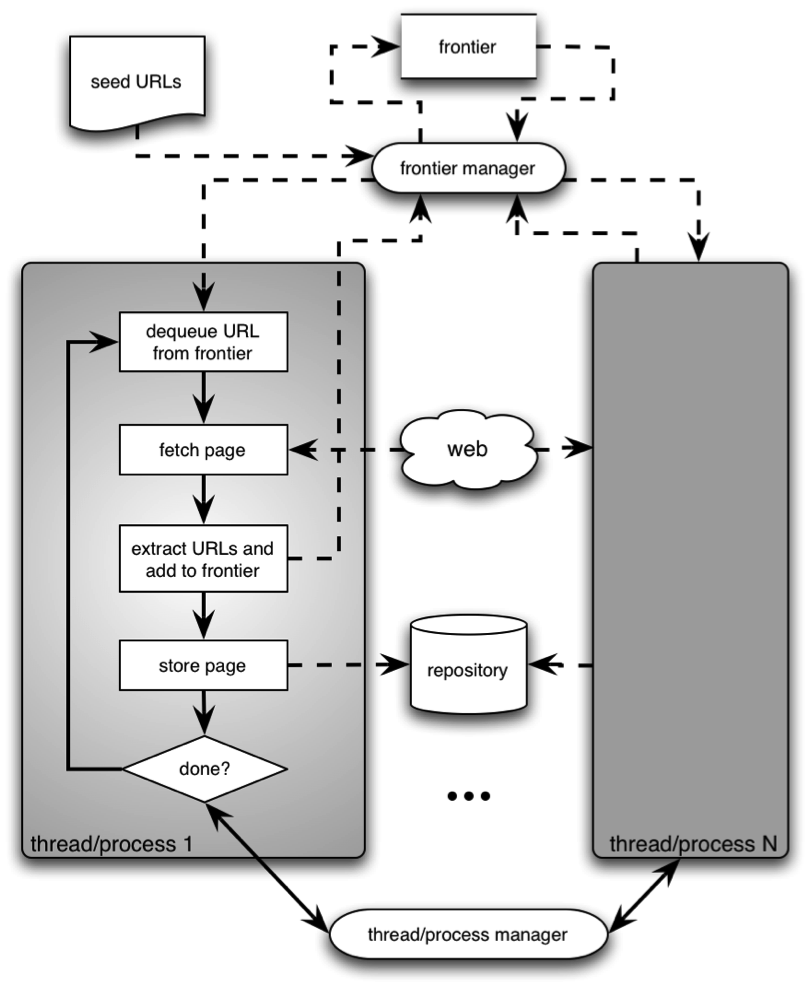
\includegraphics[width=6cm]{concurrent-crawler-arch}

\end{frame}

\begin{frame} \frametitle{Concurrent Crawlers}
\begin{itemize}
\item Can use multi-processing or multi-threading
\item Each process or thread works like a sequential crawler, except they share data structures: frontier and repository
\item Shared data structures must be synchronized (locked for concurrent writes)
\item Speedup of factor of 5-10 are easy this way
\end{itemize}

\end{frame}


\section{Universal Crawlers}


\begin{frame} \frametitle{Universal Crawlers}

\begin{itemize}

\item Support universal search engines

\item Large-scale

\item Huge cost (network bandwidth) of crawl is amortized over many queries from users

\item Incremental updates to existing index and other data repositories
\end{itemize}


\end{frame}

\begin{frame} \frametitle{Universal Crawlers}


\begin{block}{Two major issues:}

\begin{description}
\item[Performance:] Need to scale up to billions of pages
\item[Policy:] Need to trade-off coverage, freshness, and bias (e.g. toward ``important'' pages)
\end{description}

\end{block}

\end{frame}


\begin{frame} \frametitle{Large-Scale Crawlers: Performance and Scalability}

\begin{block}{Issues:}
\begin{itemize}
  \item Need to minimize overhead of DNS lookups
  \item Need to optimize utilization of network bandwidth and disk
    throughput (I/O is bottleneck) 
    \begin{itemize}
        \item Multi-processing or multi-threading do not scale up to billions of pages
    \end{itemize}
\end{itemize}
\end{block}

\begin{block}{Use asynchronous sockets}


Non-blocking: hundreds of network connections open simultaneously

Polling socket to monitor completion of network transfers
\end{block}

\end{frame}

\begin{frame} \frametitle{High-level Architecture of a \\ Scalable Universal Crawler}

      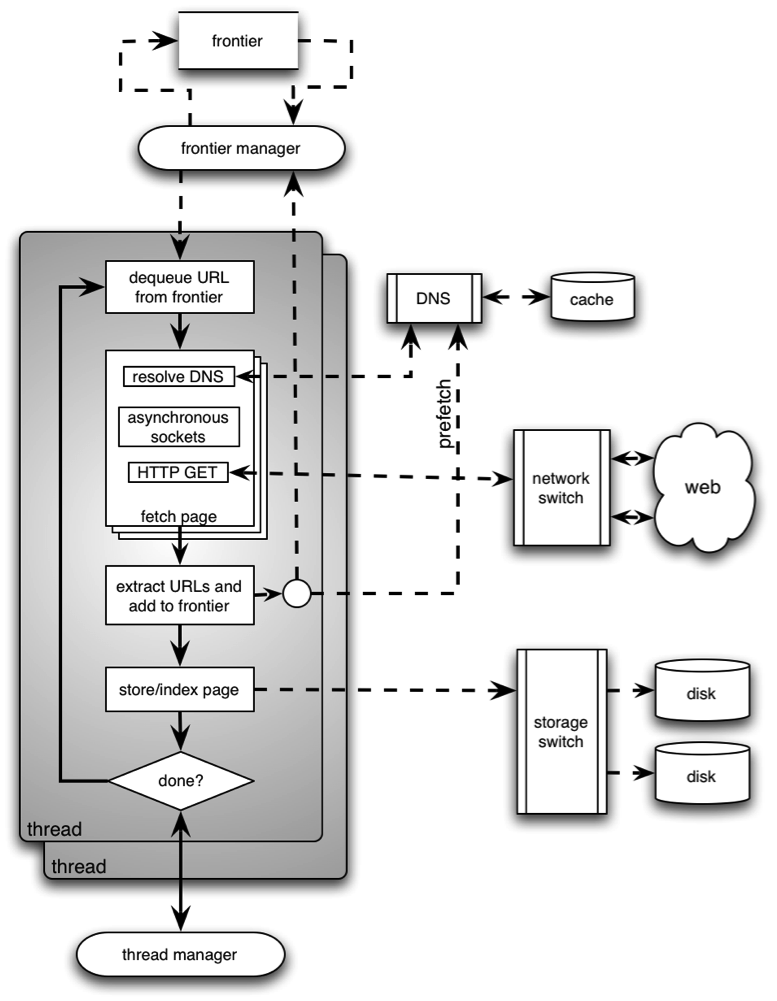
\includegraphics[width=6cm]{scalable-crawler-arch}

\end{frame}


\begin{frame} \frametitle{Universal Crawlers: Policy}


Two main requirements must be met:

  \begin{columns}[T]
    \begin{column}{0.5\textwidth}
\textbf{Coverage}

\begin{itemize}
   \item New pages get added all the time
   \item Can the crawler find every page?
\end{itemize}
 
    \end{column}
    \begin{column}{0.5\textwidth}

\textbf{Freshness}

\begin{itemize}
\item Pages change over time, get removed, etc.
\item How frequently can a crawler revisit ?
\end{itemize}

   \end{column}
\end{columns}

\vfill

\begin{block}{Trade-off!}
Focus on most ``important'' pages (crawler bias)

``Importance'' is subjective
\end{block}

\end{frame}

\begin{frame} \frametitle{Maintaining a ``fresh'' collection}

Universal crawlers are never ``done''

High variance in rate and amount of page changes

HTTP headers are notoriously unreliable
\begin{itemize}
\item Last-modified
\item Expires
\end{itemize}


\begin{block}{Solution}
\begin{itemize}
\item Estimate the probability that a previously visited page has changed in the meanwhile
\item Prioritize by this probability estimate
\end{itemize}
\end{block}

\end{frame}

\begin{frame} \frametitle{Estimating Page Change Rates}

Algorithms for maintaining a crawl in which most pages are fresher than a specified epoch
%\begin{itemize} \item Brewington \& Cybenko; Cho, Garcia-Molina \&
%  Page \end{itemize}

\vfill
\begin{block}{Assumption: recent past predicts the future} 

(Ntoulas, Cho \& Olston 2004)

\begin{itemize}
\item Frequency of change not a good predictor
\item Degree of change is a better predictor
\end{itemize}
\end{block}

\end{frame}


\begin{frame} \frametitle{Do We Need to Crawl the Entire Web?}
If we cover too much, it will get stale

There is an abundance of pages in the Web

For PageRank, pages with very low prestige are largely  useless

\begin{block}{What is the goal?}

\begin{itemize}
\item General search engines: pages with high prestige 
\item News portals: pages that change often
\item Vertical portals: pages on some topic
\end{itemize}
\end{block}


%What are appropriate priority measures in these cases? Approximations?
\end{frame}

\section{Preferential Crawlers}


\begin{frame} \frametitle{Breadth-first Crawlers}

BF crawler tends to crawl high-PageRank pages very early

%Therefore, BF crawler is a good baseline to gauge other crawlers

But why is this so?

\end{frame}

\begin{frame} \frametitle{Bias of Breadth-first Crawlers}

%% could introduce here some detail on the strcuture of the web 
%% http://www.slideshare.net/olyerickson/itws-1100-whatiswebsciencefinal

\begin{block}{The structure of the Web graph is very different from a random network}

\begin{itemize}
\item Scale-free network: Power-law distribution of in-degree
\item There are hub pages with very high PR and many incoming links
\begin{itemize}
\item These are attractors: you cannot avoid them!
\end{itemize}
\end{itemize}

\end{block}

\end{frame}


\begin{frame} \frametitle{Preferential Crawlers}

Assume we can estimate for each page an {\em importance measure}, $I(p)$

Want to visit pages in order of decreasing $I(p)$

Maintain the frontier as a priority queue sorted by $I(p)$


\end{frame}


\begin{frame} \frametitle{Preferential Crawlers}

Selective bias toward some pages, eg. most ``relevant''/topical, closest to seeds, most popular/largest PageRank, unknown servers, highest rate/amount of change, etc...

\begin{block}{Focused crawlers}
Supervised learning: classifier based on labeled examples drives the
crawler frontier
\end{block}


\begin{block}{Topical crawlers}

Best-first search based on $similarity(topic, parent)$
\end{block}

\begin{block}{Adaptative crawlers}
\begin{itemize}
  \item Reinforcement learning
  \item Evolutionary algorithms/artificial life
\end{itemize}
\end{block}

\end{frame}




\begin{frame} \frametitle{Preferential Crawling Algorithms: Examples}

\begin{description}
%\item [Breadth-First:] Exhaustively visit all links in order encountered
\item [Best-N-First: ] Priority queue sorted by preference, explore top N at a time %\\
%Variants: DOM context, hub scores
\item [PageRank:] Priority queue sorted by PageRank
\item [SharkSearch:] Priority queue sorted by combination of
  similarity, anchor text, similarity of parent, etc. %% (powerful cousin of FishSearch)
\item[InfoSpiders:] Adaptive distributed algorithm using an evolving population of learning agents
\end{description}
\end{frame}


\begin{frame} \frametitle{Preferential Crawlers: PageRank to
    Prioritize Crawl}

  \begin{columns}[T]

    \begin{column}{0.4\textwidth}

For I(p) = PageRank \\
 (estimated based on pages crawled so far), \\
we can {\bf find high backlink pages faster} than a breadth-first crawler. 

    \end{column}

    \begin{column}{0.6\textwidth}
     
     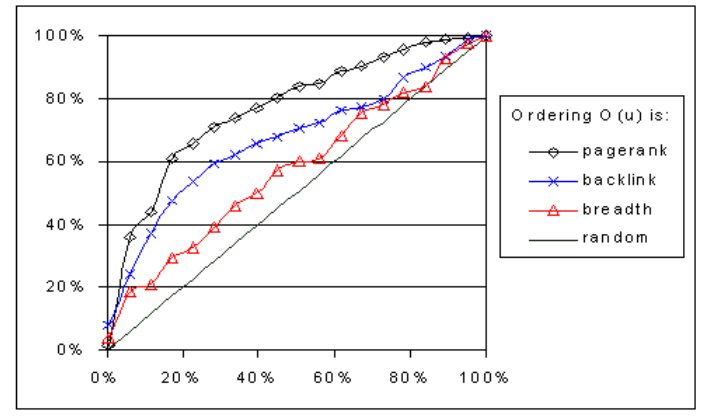
\includegraphics[width=\textwidth]{cho-molina-focused-crawlers}
     \small{ \%  pages crawled with backlinks above 100 as function of \% of pages crawled.}

    \end{column}

\end{columns}

\vfill

\small{Cho, Garcia-Molina \& Page, {\em Efficient Crawling Through URL
  Ordering}, WWW 1998. \url{http://ilpubs.stanford.edu:8090/347/1/1998-51.pdf}}

\end{frame}


\begin{frame} \frametitle{Preferential Crawlers: Figures of Merit}

\begin{equation*}
Precision \approx \frac{| p: crawled(p) \wedge I(p) > threshold |} {| p: crawled(p) |}
\end{equation*}
\vfill
\begin{equation*}
Recall \approx  \frac{| p: crawled(p) \wedge I(p) > threshold |}{ | p: I(p) > threshold|}
\end{equation*}

\end{frame}



\begin{frame} \frametitle{Focused Crawlers: Basic Idea}


\begin{columns}
\begin{column}{0.7\textwidth}

Train Na\"ive-Bayes classifier based on example pages in desired set of
topics, $c*$. For each class $c \in c*$ we compute a Score
for $p$ 
\begin{equation*}
Pr(c*|p) = \sum_{c \in c*} Pr(c|p)
\end{equation*}

Decision is based on defined threshold.
\end{column}
\begin{column}{0.3\textwidth}

\begin{center}
     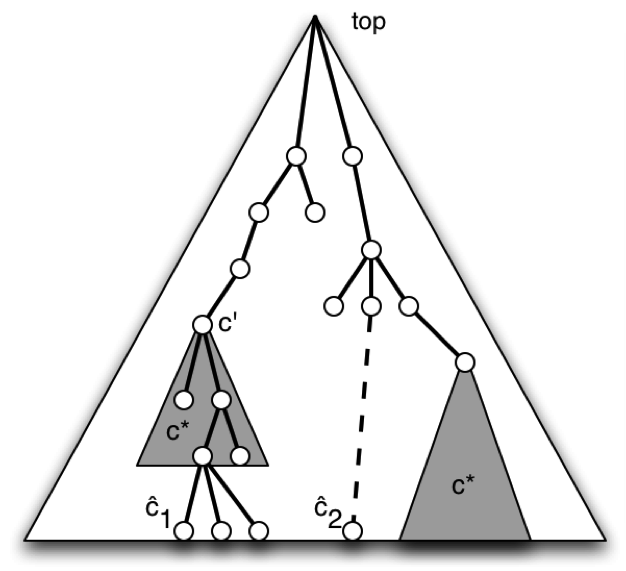
\includegraphics[width=\textwidth]{ODP}

The ODP topic hierarchy
\end{center}

\end{column}

\end{columns}

\end{frame}


% \begin{frame} \frametitle{Focused Crawlers: Soft vs. Hard Focus}

% \begin{columns}
% \begin{column}{0.5\textwidth}

% \begin{block}{Soft focus:} 

% Frontier is priority queue using $Score(p)$ for each $p$

% \end{block}

% \begin{block}{Hard focus:} % http://www8.org/w8-papers/5a-search-query/crawling/
% Find best leaf $\hat{c}$ for $p$ 

% If an ancestor $c'$ of $\hat{c} $ is in $c*$ then add links from $p$ to
% frontier, else discard.


% \end{block}


% \end{column}

% \begin{column}{0.5\textwidth}

% \begin{center}
%      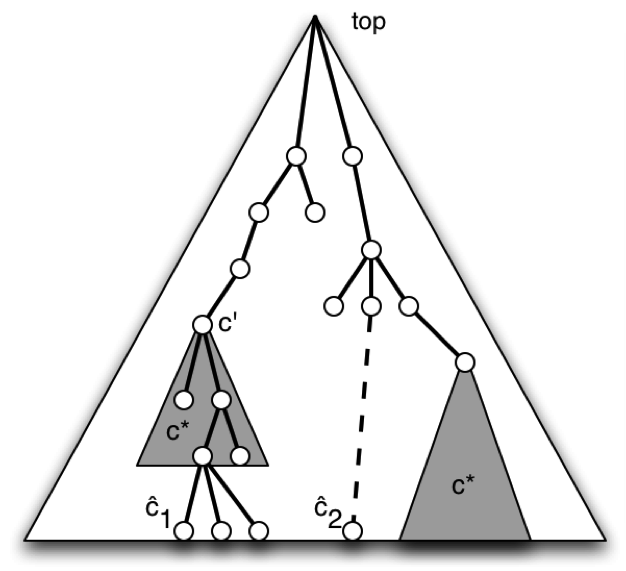
\includegraphics[width=\textwidth]{ODP}
% %The ODP topic hierarchy
% \end{center}

% \end{column}

% \end{columns}

% \vfill
% Soft and hard focus work equally well empirically

% %% When the crawler is in a “soft” focused mode, it uses the relevance
% %% score of the crawled page to score the unvisited URLs extracted
% %% from it. The scored URLs are then added to the frontier. Then in a
% %% manner similar to the naive best-first crawler, it picks the best
% %% URL to crawl next. 

% %% In the “hard” focused mode, for a crawled page p, the classifier
% %% first finds the leaf node c∗ (in the taxonomy) with maximum
% %% probability of including p. If any of the parents (in the taxonomy)
% %% of c∗ are marked as “good” by the user, then the URLs from the
% %% crawled page p are extracted and added to the frontier. 
% \end{frame}



\begin{frame} \frametitle{Focused Crawlers}

\begin{itemize}
\item Can have multiple topics with as many classifiers, with scores appropriately combined (Chakrabarti et al. 1999)

%\item Can use a {\em distiller} to find topical hubs periodically, and add these to the frontier


%% Another interesting element of the focused crawler is the use of a
%% distiller. The distiller applies a modified version of Kleinberg’s
%% algorithm [17] to find topical hubs. The hubs provide links to many
%% authoritative sources on the topic. The distiller is activated at
%% various times during the crawl and some of the top hubs are added
%% to the frontier.


% \item Can accelerate with the use of a critic (Chakrabarti et al. 2002)

\item Can use alternative classifier algorithms to naïve-Bayes.
\begin{itemize} 
  \item SVM and neural nets have reportedly performed better (Pant \&
    Srinivasan 2005)
\end{itemize}

\end{itemize}
\end{frame}



\begin{frame} \frametitle{Context-focused Crawlers}

%Same idea, but multiple classes (and classifiers). 

\begin{columns}

\begin{column}{0.6\textwidth}

\begin{itemize}
\item Classifiers trained based on link distance from relevant targets
\begin{itemize}
\item l=0 is topic of interest
\item l=1 link to topic of interest
\item Etc.
\end{itemize}

\item Initially needs a back-crawl from seeds (or known targets) to train classifiers to estimate distance
\item Links in frontier prioritized based on estimated distance from targets
\item Outperforms standard focused crawler empirically
\end{itemize}

\end{column}
\begin{column}{0.4\textwidth}

\begin{center}
     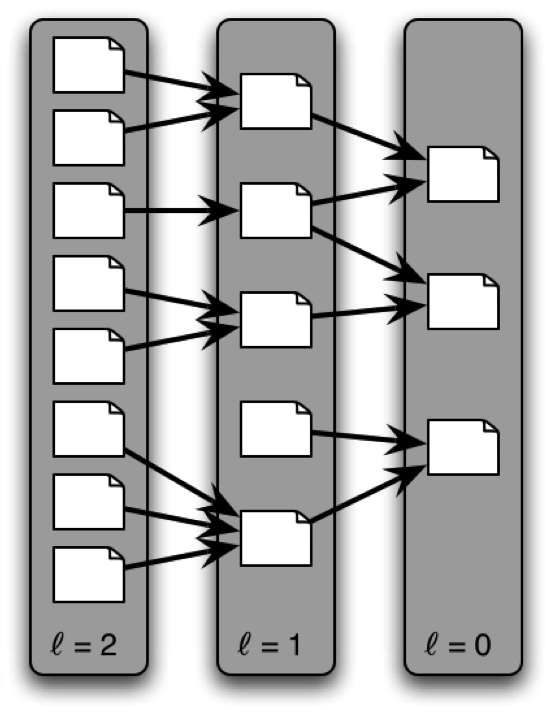
\includegraphics[width=.8\textwidth]{crawler-focused-context-graph}

Context graph with 3 layers

\end{center}

\end{column}

\end{columns}

\end{frame}



\begin{frame} \frametitle{Topical Crawlers}

\begin{block}{No labeled examples}
All we have is a topic (query, description, keywords) and a set of
seed pages (not necessarily relevant). 
\end{block}

Must predict relevance of unvisited links to prioritize

\small{Original idea: Menczer 1997, Menczer \& Belew 1998 }

\end{frame}

% \begin{frame} \frametitle{My Spiders}

% Example that no longer works:

% \url{http://myspiders.informatics.indiana.edu}

% real-time crawler: given a search query, find top-k results and crawl
% the next.

% \end{frame}


\begin{frame} \frametitle{Topical Locality}

Topical locality is a necessary condition for a topical crawler to
work, and for surfing to be a worthwhile activity for humans

Links must encode semantic information, i.e. say something about neighbor pages, not be random

It is also a sufficient condition if we start from ``good'' seed pages

Indeed we know that Web topical locality is strong :
\begin{itemize}
\item Indirectly (crawlers work and people surf the Web)
\item From direct measurements (Davison 2000; Menczer 2004, 2005)
\end{itemize}


\end{frame}


% \begin{comment}

% \begin{frame} \frametitle{ Quantifying Topical Locality}

% \begin{columns}

% \begin{column}{0.6\textwidth}

% Different ways to pose the question:
% \begin{itemize}
% \item How quickly does semantic locality decay?
% \item How fast is topic drift?
% \item How quickly does content change as we surf away from a starting
%   page?
% \end{itemize}

% \end{column}
% \begin{column}{0.4\textwidth}

% \begin{center}
%      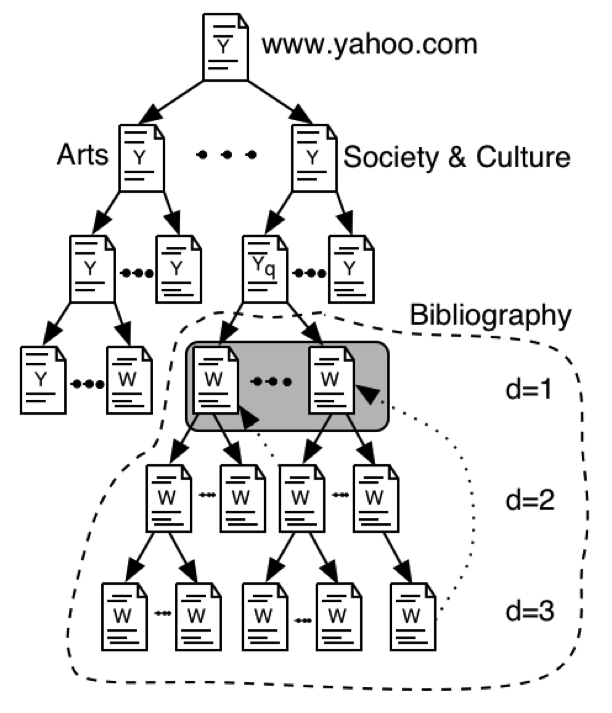
\includegraphics[width=.8\textwidth]{crawler-focused-locality}

% \end{center}

% \end{column}

% \end{columns}

% To answer these questions, let us consider exhaustive breadth-first crawls from 100 topic pages 

% \end{frame}


% \begin{frame} \frametitle{ The ``link-cluster'' conjecture}


% Connection between semantic topology (relevance) and link topology (hypertext)

% $G = Pr[rel(p)] $ \~ fraction of relevant/topical pages (topic generality)

% $R = Pr[rel(p) | rel(q) AND link(q,p)] $ \~ cond. prob. Given neighbor on topic
% Related nodes are clustered if  $R > G$

% Necessary and sufficient condition for a random crawler to find pages related to start points

% Example: 2 topical clusters with stronger modularity within each
% cluster than outside

% \end{frame}


% \begin{frame} \frametitle{ Link-cluster conjecture}

% Stationary hit rate for a random crawler:

% \end{frame}

% \begin{frame} \frametitle{ Link-cluster conjecture}

% Preservation of semantics (meaning) across links
% 1000 times more likely to be on topic if near an on-topic page!

% \end{frame}

% \begin{frame} \frametitle{ The ``link-content'' conjecture}

% Correlation of lexical (content) and linkage topology

% L(d): average link distance

% S(d): average content similarity to start (topic) page from pages up to distance $d$ 

% \begin{equation*}
% Correlation r(L,S) = -0.76
% \end{equation*}

% \end{frame}


% \begin{frame} \frametitle{ Heterogeneity of Link-Content Correlation}

% \end{frame}


% \end{comment}



% \begin{frame} \frametitle{ Topical locality-inspired tricks for topical crawlers}

% \begin{columns}

% \begin{column}{0.4\textwidth}

% {\bf Co-citation (a.k.a. sibling locality):}A and C are good hubs,
% thus A and D should be given high priority \\
% {\bf Co-reference (a.k.a. blbliographic coupling):} E and G are good
%   authorities, thus E and H should be given high priority

% \end{column}
% \begin{column}{0.6\textwidth}

% \begin{center}
%      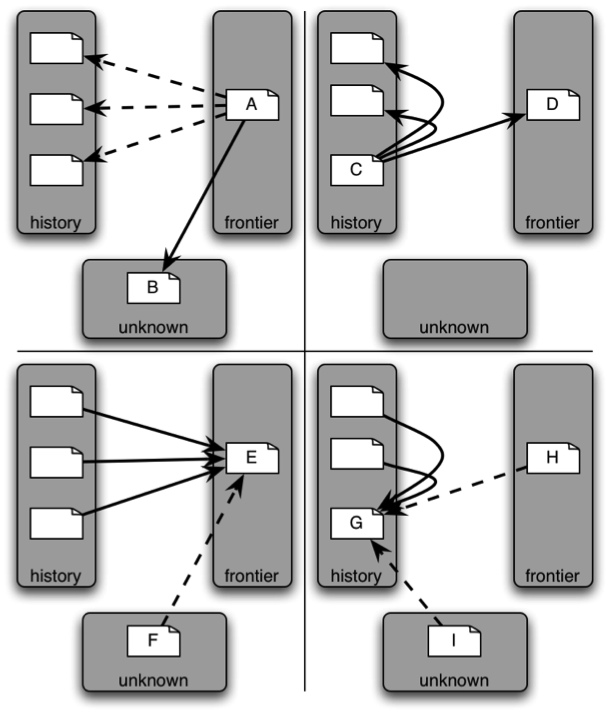
\includegraphics[width=.9\textwidth]{crawler-focused-cocite-coref}
% \end{center}

% \end{column}

% \end{columns}

% \end{frame}


% \begin{frame} \frametitle{ Correlations between Different Similarity
%     Measures}


% Semantic similarity measured from ODP, correlated with:
% \begin{description}
% \item [Content similarity:] TF or TF-IDF vector cosine
% \item [Link similarity:] Jaccard coefficient of (in+out) link neighborhoods
% \end{description}

% \begin{columns}

% \begin{column}{0.5\textwidth}
% Correlation overall is significant but weak (compare to ``All Pairs'')

% Much stronger topical locality in some topics, e.g.:
% \begin{itemize}
% \item Links very informative in news sources
% \item Text very informative in recipes
% \end{itemize}

% \end{column}
% \begin{column}{0.5\textwidth}

% \begin{center}
%      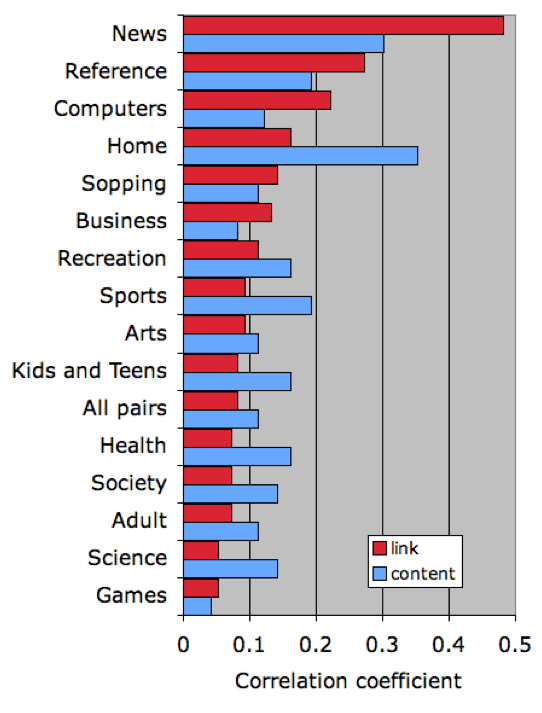
\includegraphics[width=.9\textwidth]{crawler-focused-correlations}
% \end{center}

% \end{column}

% \end{columns}


% \end{frame}





\begin{frame}[fragile] \frametitle{ Simplest topical crawler: Na\"ive
    Best-First }
{\small
\begin{verbatim}
BestFirst(topic, seed_urls) {
   foreach link (seed_urls) {
      enqueue(frontier, link);
   }
   while (len(frontier) > 0 and visited < MAX_PAGES) {
      link := dequeue_link_with_max_score(frontier);
      doc := fetch_new_document(link);
      score :=  sim(topic, doc);
      foreach outlink (extract_links(doc)) {
         if (len(frontier) >= MAX_BUFFER) {
            dequeue_link_with_min_score(frontier);
         }
         enqueue(frontier, outlink, score);
} } }
\end{verbatim}
}

\begin{block}{}
Frontier is priority queue based on text similarity between topic and
parent page.
\end{block}

\end{frame}


\begin{frame} \frametitle{Best-first Variations}
 
Correspond to different ways to score unvisited URLs: 

\begin{itemize}
\item Giving more importance to certain HTML markup in parent page
\item Extending text representation of parent page with anchor text from ``grandparent'' pages 
\item Limiting link context to less than entire page
\item Exploiting topical locality (co-citation)
%\item Exploration vs exploitation: relax priorities
\end{itemize}

\begin{block}{}
Any of these can be (and many have been) combined
\end{block}

\end{frame}



% \begin{frame} \frametitle{Link context based on text neighborhood}
 
% Often consider a fixed-size window, e.g. 50 words around anchor

% Can weigh links based on their distance from topic keywords within the
% document %% (InfoSpiders, Clever)

% Anchor text deserves extra importance

% \end{frame}

% \begin{frame} \frametitle{Link context based on DOM tree}
 

% Consider DOM subtree rooted at parent node of link's $<a>$ tag

% Or can go further up in the tree (Naïve Best-First is special case of entire document body)

% %% Trade-off between noise due to too small or too large context tree (Pant 2003)
% \end{frame}
 


% \begin{comment}

% \begin{frame} \frametitle{DOM context}
 
% xxxx
% \end{frame}


% \begin{frame} \frametitle{ Co-citation: hub scores}

% xxxx
% \end{frame}

% \begin{frame} \frametitle{ Combining DOM context and hub scores}

% xxx

% \end{frame}
 

% \end{comment}

% \begin{frame} \frametitle{ Exploration vs Exploitation}

% \begin{block}{Best-N-First (or BFSN)}
% Rather than re-sorting the frontier every time you add links, \\
% be lazy and sort only every N pages visited 
% \end{block}

% Empirically, being less greedy helps crawler performance significantly: escape ``local topical traps'' by exploring more.
% \end{frame}
 

% \begin{comment}
% \begin{frame} \frametitle{ InfoSpiders}
% A series of intelligent multi-agent topical crawling algorithms employing various adaptive techniques:
% \begin{itemize}
% \item Evolutionary bias of exploration/exploitation
% \item Selective query expansion
% \item (Connectionist) reinforcement learning
% \end{itemize}
% \end{frame}
 

% \begin{frame} \frametitle{ Link scoring and selection by each crawling agent}
% xxxx
% \end{frame}

% \begin{frame} \frametitle{XXXX}
% xxxx
% \end{frame}

% \begin{frame} \frametitle {Adaptation in InfoSpiders}

% Unsupervised population evolution
% \begin{itemize}
% \item Select agents to match resource bias
% \item Mutate internal queries: selective query expansion
% \item Mutate weights
% \end{itemize}

% Unsupervised individual adaptation
% \begin{itemize}
% \item Q-learning: adjust neural net weights to predict relevance
%   locally
% \end{itemize}

% \end{frame}

% \begin{frame} \frametitle{Infospiders}

% InfoSpiders evolutionary bias: an agent in a relevant area will spawn other agents to exploit/explore that neighborhood

% \end{frame}



% \begin{frame} \frametitle{ Multithreaded InfoSpiders (MySpiders)}

% Different ways to compute the cost of visiting a document:
% \begin{description}
% \item [Constant:] $cost_{const} = E_0 p_0 / T_{max}$

% \item [Proportional to download time:] $cost_{time} = f(cost_{const} t / timeout)$
% \end{description}

% The latter is of course more efficient (faster crawling), but it also yields better quality pages!
% \end{frame}



% \begin{frame} \frametitle{Selective Query Expansion in InfoSpiders: \\Internalization of local text features}
 
% When a new agent is spawned, it picks up a common term from the current page (here 'th')

% \end{frame}
 

% \begin{frame} \frametitle{Reinforcement Learning}

% In general, reward function R: S A 

% Learn policy (: S A) to maximize reward over time, typically discounted in the future:

% Q-learning: optimal policy 

% \end{frame}
 
% \begin{frame} \frametitle{Q-learning in InfoSpiders}

% Use neural nets to estimate Q scores

% Compare estimated relevance of visited page with Q score of link
% estimated from parent page to obtain feedback signal

% Learn neural net weights using back-propagation of error with teaching
% input: $ E(D) +  maxl(D) l $
% \end{frame}
 

% \begin{frame} \frametitle{Other Reinforcement Learning Crawlers}

% Rennie \& McCallum (1999): 
% \begin{itemize}
% \item Naïve-Bayes classifier trained on text nearby links in pre-labeled examples to estimate Q values
% \item Immediate reward R=1 for ``on-topic'' pages (with desired CS papers for CORA repository)
% \item All RL algorithms outperform Breath-First Search
% \end{itemize}

% Future discounting: ``For spidering, it is always better to choose immediate over delayed rewards'' -- Or is it?
% \begin{itemize}
% \item But we cannot possibly cover the entire search space, and recall that by being greedy we can be trapped in local topical clusters and fail to discover better ones

% \item Need to explore!

% \end{itemize}

% \end{frame}

% \end{comment}


% \section{Evaluation of preferential crawlers}


% \begin{frame} \frametitle{Evaluation of Topical Crawlers}


% Goal: build ``better'' crawlers to support applications (Srinivasan \& al. 2005) 

% Build an unbiased evaluation framework

% Define common tasks of measurable difficulty

% Identify topics, relevant targets

% \begin{block}{Identify appropriate performance measures}

% \begin{description}
% \item[Effectiveness:] quality of crawler pages, order, etc.

% \item [Efficiency:] separate CPU \& memory of crawler algorithms from
%   bandwidth \& common utilities
% \end{description}
% \end{block}

% \end{frame}


% \begin{frame} \frametitle{Evaluation corpus = ODP + Web}



% \begin{center}
%      
\includegraphics[width=.8\textwidth]{Dmoz_open_directory_thumb}
% \end{center}

% \begin{center}
% \url{http://www.dmoz.org}
% \end{center}

% \end{frame}


% \begin{frame} \frametitle{Topics and Targets}


% \begin{center}
%      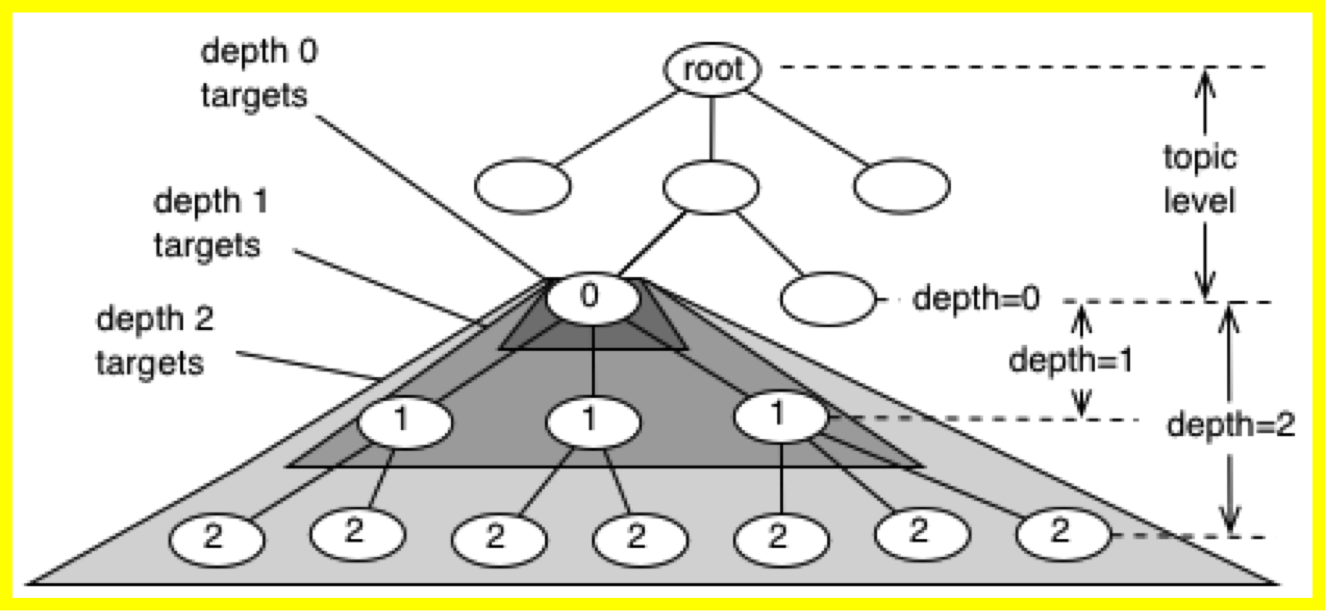
\includegraphics[width=.8\textwidth]{topics-targets}
% \end{center}


% topic level $\sim$ specificity

% depth $\sim$ generality
% \end{frame}



% \begin{frame} \frametitle{Tasks}

% \begin{center}
%      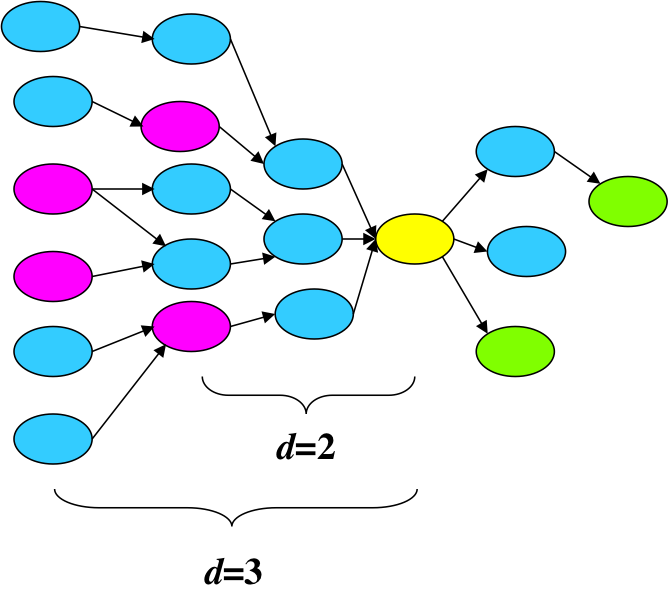
\includegraphics[width=.4\textwidth]{evaluation-backcrawl}
% \end{center}

% {\small
% \begin{block}{}
% Start from seeds (purple), find targets (yellow) and/or pages similar
% to target descriptions (green) 
% \end{block}

% \begin{block}{Which seeds?}
% To make sure that targets are reachable, back-crawl from targets to
% get the seeds
% \end{block}
% }

% \end{frame}


% \begin{frame} \frametitle{Target based performance measures}

% \begin{center}
%      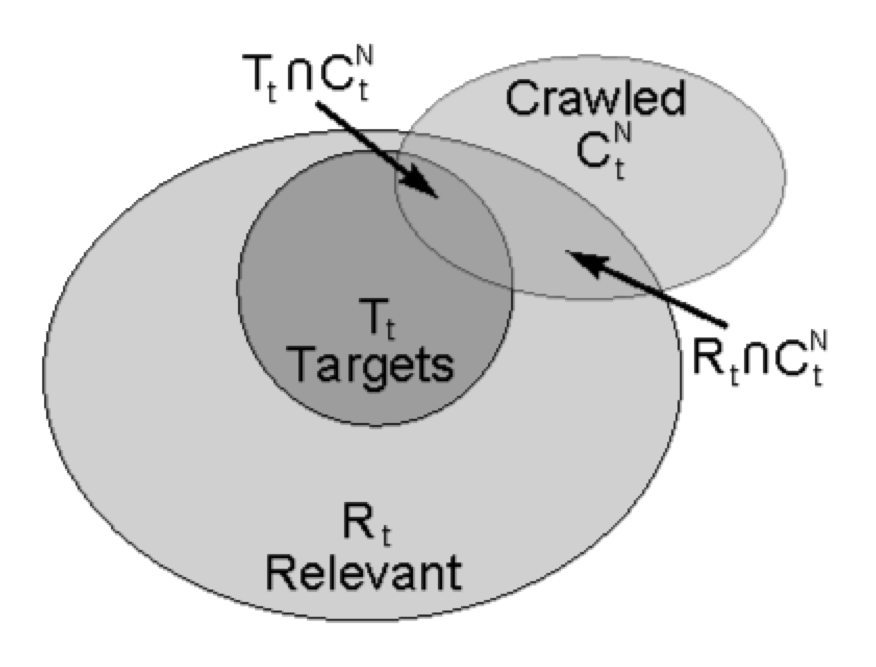
\includegraphics[width=.8\textwidth]{target-based-metrics}
% \end{center}
% \end{frame}

% \begin{frame} \frametitle{Alternative: split targets in two sets}

% Performance matrix

% \begin{center}
%      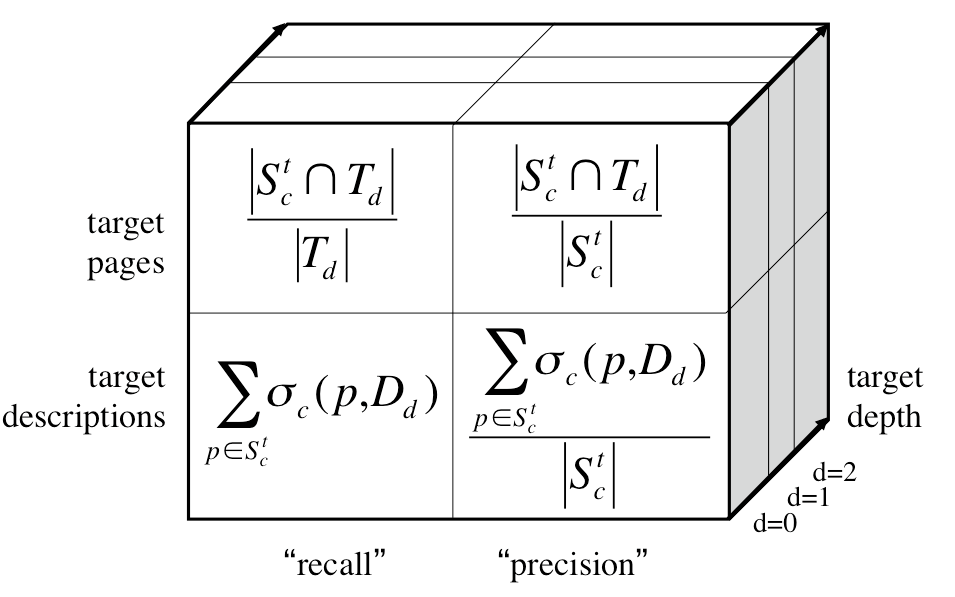
\includegraphics[width=.8\textwidth]{performance-matrix}
% \end{center}

% \end{frame} 


% \begin{comment}

% \begin{frame} \frametitle{Crawling evaluation framework}

% \end{frame} 


% \begin{frame} \frametitle{Using framework to compare crawler performance}

% \end{frame} 


% \begin{frame} \frametitle{Efficiency \& scalability}

% \end{frame} 




% \begin{frame} \frametitle{Topical Crawler  Performance depends on Topic Characteristics}

% \end{frame} 


% \end{comment}



\section{Crawler ethics and conflicts}


\begin{frame} \frametitle{Crawler ethics and Conflicts}


Crawlers can cause trouble, even unwillingly, if not properly designed to be ``polite'' and ``ethical''

For example, sending too many requests in rapid succession to a single server can amount to a Denial of Service (DoS) attack!
\begin{itemize}
\item Server administrator and users will be upset
\item Crawler developer/admin IP address may be blacklisted
\end{itemize}
\end{frame}


\begin{frame} \frametitle{Crawler Etiquette (important!)}

Identify yourself
\begin{itemize}
\item Use User-Agent HTTP header to identify crawler, website with description of crawler and contact information for crawler developer
\item Use From HTTP header to specify crawler developer email
\item Do not disguise crawler as a browser by using their User-Agent string
\end{itemize}

Always check that HTTP requests are successful, and in case of error, use HTTP error code to determine and immediately address problem

Pay attention to anything that may lead to too many requests to any one server, even unwillingly, e.g.:
\begin{itemize}
\item redirection loops
\item spider traps
\end{itemize}

\end{frame}



\begin{frame} \frametitle{Crawler Etiquette (important!)}

\begin{block}{Spread the load, do not overwhelm a server}
\begin{itemize}
\item Make sure that no more than some max. number of requests to any single
server per unit time, say less than 1/second
\end{itemize}
\end{block}

\begin{block}{Honor the Robot Exclusion Protocol}
\begin{itemize}

\item A server can specify which parts of its document tree any crawler is or is not allowed to crawl by a file named \url{robots.txt} placed in the HTTP root directory, e.g. \url{http://www.ist.utl.pt/robots.txt}, \url{http://www.google.com/robots.txt}

\item Crawler should always check, parse, and obey this file before sending any requests to a server

\item More info at:

\url{http://www.robotstxt.org/wc/exclusion.html}

\end{itemize}

\end{block}

\end{frame}


\begin{frame} \frametitle{More on Robot Exclusion}

\begin{itemize}
\item Make sure URLs are canonical before checking against {\tt robots.txt} 

\item Avoid fetching {\tt robots.txt} for each request to a server by
  caching its policy as relevant to this crawler

\item {\tt Sitemap} and {\tt sitemap.xml} may help (e.g. \url{https://support.google.com/webmasters/answer/183668?hl=en})

\item Let's look at some examples to understand the protocol

\end{itemize}
\end{frame}

\begin{frame}[fragile] \frametitle{Apple.com}

\begin{block}{\url{http://www.apple.com/robots.txt}}
\end{block}

\begin{verbatim}
# robots.txt for http://www.apple.com/
User-agent: *
Disallow: 
\end{verbatim}

everyone welcome to crawl anything they want!

\end{frame}

\begin{frame}[fragile] \frametitle{IST.UTL.PT}

\begin{block}{\url{http://www.ist.utl.pt/robots.txt}}
\end{block}

\begin{verbatim}

User-agent: *
Disallow: /img/
Disallow: /css/
Disallow: /inc/
Disallow: /lib/
Disallow: /newscache/
Disallow: /researchersCache/
\end{verbatim}

everyone welcome to crawl anything except specified directories.

\end{frame}


% \begin{frame}[fragile] \frametitle{ACM.org}

% \begin{block}{\url{http://www.acm.org/robots.txt}}

% \end{block}

% \begin{verbatim}


% \end{verbatim}


% \end{frame}



% \begin{frame}[fragile] \frametitle{Microsoft.com}

% \begin{block}{\url{http://www.microsoft.com/robots.txt}}

% \end{block}

% \begin{verbatim}


% \end{verbatim}


% \end{frame}
 
% \begin{frame}[fragile] \frametitle{Springer.com}

% \begin{block}{\url{http://www.springer.com/robots.txt}}

% \end{block}


% \begin{verbatim}


% \end{verbatim}



% \end{frame}
 
\begin{frame} \frametitle{Robots.txt Compliance}

\begin{block}{Is compliance with robot exclusion a matter of law? }

No! Compliance is voluntary, but if you do not comply, you may be blocked

Someone (unsuccessfully) \href{http://www.theregister.co.uk/2007/07/26/wayback_firm_suit/}{sued Internet Archive} over a {\tt robots.txt} related issue

\end{block}
\end{frame}


\begin{frame} \frametitle{Disguised Crawlers}

\begin{block}{Some crawlers Disguise Themselves}

Using false User-Agent 

Randomizing access frequency to look like a human/browser

Why? Example: click fraud for ads

\end{block}

\end{frame}

\begin{frame} \frametitle{Disguised Servers}

\begin{block}{Cloaking:} 
present different content based on User-Agent

E.g. stuff keywords on version of page shown to search engine crawler
\end{block}

Search engines do not look kindly on this type of ``spamdexing'' and remove from their index sites that perform such abuse

\vfill

Case of bmw.de made the news: \url{http://en.wikipedia.org/wiki/Spamdexing}
\end{frame}

\begin{frame} \frametitle{Gray Areas for Crawler Ethics }

If you write a crawler that unwillingly follows links to ads, are you
just being careless, or are you violating terms of service, or are you
violating the law by defrauding advertisers?
\begin{itemize}
\item Is non-compliance with Google's \url{robots.txt} in this case equivalent to click fraud?
\end{itemize}

If you write a browser extension that performs some useful service, should you comply with robot exclusion?
\end{frame}


%This section of the chapter will be skipped.
%\section{New developments}

% \begin{frame} \frametitle{Social, Collaborative, Federated Crawlers}

% \begin{itemize}
% \item Idea: go beyond the ``one-fits-all'' model of centralized search engines

% \item Extend the search task to anyone, and distribute the crawling task

% \item Each search engine is a peer agent

% \item Agents collaborate by routing queries and results
% \end{itemize}

% \end{frame}


\begin{frame} \frametitle{Need Crawling Code?}

\begin{itemize}
\item Just google ``python crawler''
\item Large-scale open source crawlers:
\begin{description}
\item [Nutch:] \url{http://nutch.apache.org/}
\item [Heritrix:] \url{http://crawler.archive.org/}
\end{description}

\end{itemize}
\end{frame}


% ------------------------------------------------------------
% ------------------------------------------------------------

\finalframe{Questions?}

\end{document}
